
%% bare_conf.tex
%% V1.4b
%% 2015/08/26
%% by Michael Shell
%% See:
%% http://www.michaelshell.org/
%% for current contact information.
%%
%% This is a skeleton file demonstrating the use of IEEEtran.cls
%% (requires IEEEtran.cls version 1.8b or later) with an IEEE
%% conference paper.
%%
%% Support sites:
%% http://www.michaelshell.org/tex/ieeetran/
%% http://www.ctan.org/pkg/ieeetran
%% and
%% http://www.ieee.org/

%%*************************************************************************
%% Legal Notice:
%% This code is offered as-is without any warranty either expressed or
%% implied; without even the implied warranty of MERCHANTABILITY or
%% FITNESS FOR A PARTICULAR PURPOSE! 
%% User assumes all risk.
%% In no event shall the IEEE or any contributor to this code be liable for
%% any damages or losses, including, but not limited to, incidental,
%% consequential, or any other damages, resulting from the use or misuse
%% of any information contained here.
%%
%% All comments are the opinions of their respective authors and are not
%% necessarily endorsed by the IEEE.
%%
%% This work is distributed under the LaTeX Project Public License (LPPL)
%% ( http://www.latex-project.org/ ) version 1.3, and may be freely used,
%% distributed and modified. A copy of the LPPL, version 1.3, is included
%% in the base LaTeX documentation of all distributions of LaTeX released
%% 2003/12/01 or later.
%% Retain all contribution notices and credits.
%% ** Modified files should be clearly indicated as such, including  **
%% ** renaming them and changing author support contact information. **
%%*************************************************************************


% *** Authors should verify (and, if needed, correct) their LaTeX system  ***
% *** with the testflow diagnostic prior to trusting their LaTeX platform ***
% *** with production work. The IEEE's font choices and paper sizes can   ***
% *** trigger bugs that do not appear when using other class files.       ***                          ***
% The testflow support page is at:
% http://www.michaelshell.org/tex/testflow/



\documentclass[conference]{../sty/IEEEtran}
% Some Computer Society conferences also require the compsoc mode option,
% but others use the standard conference format.
%
% If IEEEtran.cls has not been installed into the LaTeX system files,
% manually specify the path to it like:
% \documentclass[conference]{../sty/IEEEtran}





% Some very useful LaTeX packages include:
% (uncomment the ones you want to load)


% *** MISC UTILITY PACKAGES ***
%
%\usepackage{ifpdf}
% Heiko Oberdiek's ifpdf.sty is very useful if you need conditional
% compilation based on whether the output is pdf or dvi.
% usage:
% \ifpdf
%   % pdf code
% \else
%   % dvi code
% \fi
% The latest version of ifpdf.sty can be obtained from:
% http://www.ctan.org/pkg/ifpdf
% Also, note that IEEEtran.cls V1.7 and later provides a builtin
% \ifCLASSINFOpdf conditional that works the same way.
% When switching from latex to pdflatex and vice-versa, the compiler may
% have to be run twice to clear warning/error messages.






% *** CITATION PACKAGES ***
%
\usepackage{cite}
% cite.sty was written by Donald Arseneau
% V1.6 and later of IEEEtran pre-defines the format of the cite.sty package
% \cite{} output to follow that of the IEEE. Loading the cite package will
% result in citation numbers being automatically sorted and properly
% "compressed/ranged". e.g., [1], [9], [2], [7], [5], [6] without using
% cite.sty will become [1], [2], [5]--[7], [9] using cite.sty. cite.sty's
% \cite will automatically add leading space, if needed. Use cite.sty's
% noadjust option (cite.sty V3.8 and later) if you want to turn this off
% such as if a citation ever needs to be enclosed in parenthesis.
% cite.sty is already installed on most LaTeX systems. Be sure and use
% version 5.0 (2009-03-20) and later if using hyperref.sty.
% The latest version can be obtained at:
% http://www.ctan.org/pkg/cite
% The documentation is contained in the cite.sty file itself.






% *** GRAPHICS RELATED PACKAGES ***
%
\ifCLASSINFOpdf
  \usepackage[pdftex]{graphicx}
  % declare the path(s) where your graphic files are
  % \graphicspath{{../pdf/}{../jpeg/}}
  % and their extensions so you won't have to specify these with
  % every instance of \includegraphics
  \DeclareGraphicsExtensions{.pdf,.jpeg,.png}
\else
  % or other class option (dvipsone, dvipdf, if not using dvips). graphicx
  % will default to the driver specified in the system graphics.cfg if no
  % driver is specified.
  % \usepackage[dvips]{graphicx}
  % declare the path(s) where your graphic files are
  % \graphicspath{{../eps/}}
  % and their extensions so you won't have to specify these with
  % every instance of \includegraphics
  % \DeclareGraphicsExtensions{.eps}
\fi
% graphicx was written by David Carlisle and Sebastian Rahtz. It is
% required if you want graphics, photos, etc. graphicx.sty is already
% installed on most LaTeX systems. The latest version and documentation
% can be obtained at: 
% http://www.ctan.org/pkg/graphicx
% Another good source of documentation is "Using Imported Graphics in
% LaTeX2e" by Keith Reckdahl which can be found at:
% http://www.ctan.org/pkg/epslatex
%
% latex, and pdflatex in dvi mode, support graphics in encapsulated
% postscript (.eps) format. pdflatex in pdf mode supports graphics
% in .pdf, .jpeg, .png and .mps (metapost) formats. Users should ensure
% that all non-photo figures use a vector format (.eps, .pdf, .mps) and
% not a bitmapped formats (.jpeg, .png). The IEEE frowns on bitmapped formats
% which can result in "jaggedy"/blurry rendering of lines and letters as
% well as large increases in file sizes.
%
% You can find documentation about the pdfTeX application at:
% http://www.tug.org/applications/pdftex





% *** MATH PACKAGES ***
%
%\usepackage{amsmath}
% A popular package from the American Mathematical Society that provides
% many useful and powerful commands for dealing with mathematics.
%
% Note that the amsmath package sets \interdisplaylinepenalty to 10000
% thus preventing page breaks from occurring within multiline equations. Use:
%\interdisplaylinepenalty=2500
% after loading amsmath to restore such page breaks as IEEEtran.cls normally
% does. amsmath.sty is already installed on most LaTeX systems. The latest
% version and documentation can be obtained at:
% http://www.ctan.org/pkg/amsmath





% *** SPECIALIZED LIST PACKAGES ***
%
%\usepackage{algorithmic}
% algorithmic.sty was written by Peter Williams and Rogerio Brito.
% This package provides an algorithmic environment fo describing algorithms.
% You can use the algorithmic environment in-text or within a figure
% environment to provide for a floating algorithm. Do NOT use the algorithm
% floating environment provided by algorithm.sty (by the same authors) or
% algorithm2e.sty (by Christophe Fiorio) as the IEEE does not use dedicated
% algorithm float types and packages that provide these will not provide
% correct IEEE style captions. The latest version and documentation of
% algorithmic.sty can be obtained at:
% http://www.ctan.org/pkg/algorithms
% Also of interest may be the (relatively newer and more customizable)
% algorithmicx.sty package by Szasz Janos:
% http://www.ctan.org/pkg/algorithmicx




% *** ALIGNMENT PACKAGES ***
%
%\usepackage{array}
% Frank Mittelbach's and David Carlisle's array.sty patches and improves
% the standard LaTeX2e array and tabular environments to provide better
% appearance and additional user controls. As the default LaTeX2e table
% generation code is lacking to the point of almost being broken with
% respect to the quality of the end results, all users are strongly
% advised to use an enhanced (at the very least that provided by array.sty)
% set of table tools. array.sty is already installed on most systems. The
% latest version and documentation can be obtained at:
% http://www.ctan.org/pkg/array


% IEEEtran contains the IEEEeqnarray family of commands that can be used to
% generate multiline equations as well as matrices, tables, etc., of high
% quality.




% *** SUBFIGURE PACKAGES ***
\ifCLASSOPTIONcompsoc
  \usepackage[caption=false,font=normalsize,labelfont=sf,textfont=sf]{subfig}
\else
  \usepackage[caption=false,font=footnotesize]{subfig}
\fi
% subfig.sty, written by Steven Douglas Cochran, is the modern replacement
% for subfigure.sty, the latter of which is no longer maintained and is
% incompatible with some LaTeX packages including fixltx2e. However,
% subfig.sty requires and automatically loads Axel Sommerfeldt's caption.sty
% which will override IEEEtran.cls' handling of captions and this will result
% in non-IEEE style figure/table captions. To prevent this problem, be sure
% and invoke subfig.sty's "caption=false" package option (available since
% subfig.sty version 1.3, 2005/06/28) as this is will preserve IEEEtran.cls
% handling of captions.
% Note that the Computer Society format requires a larger sans serif font
% than the serif footnote size font used in traditional IEEE formatting
% and thus the need to invoke different subfig.sty package options depending
% on whether compsoc mode has been enabled.
%
% The latest version and documentation of subfig.sty can be obtained at:
% http://www.ctan.org/pkg/subfig



% *** FLOAT PACKAGES ***
%
%\usepackage{fixltx2e}
% fixltx2e, the successor to the earlier fix2col.sty, was written by
% Frank Mittelbach and David Carlisle. This package corrects a few problems
% in the LaTeX2e kernel, the most notable of which is that in current
% LaTeX2e releases, the ordering of single and double column floats is not
% guaranteed to be preserved. Thus, an unpatched LaTeX2e can allow a
% single column figure to be placed prior to an earlier double column
% figure.
% Be aware that LaTeX2e kernels dated 2015 and later have fixltx2e.sty's
% corrections already built into the system in which case a warning will
% be issued if an attempt is made to load fixltx2e.sty as it is no longer
% needed.
% The latest version and documentation can be found at:
% http://www.ctan.org/pkg/fixltx2e


%\usepackage{stfloats}
% stfloats.sty was written by Sigitas Tolusis. This package gives LaTeX2e
% the ability to do double column floats at the bottom of the page as well
% as the top. (e.g., "\begin{figure*}[!b]" is not normally possible in
% LaTeX2e). It also provides a command:
%\fnbelowfloat
% to enable the placement of footnotes below bottom floats (the standard
% LaTeX2e kernel puts them above bottom floats). This is an invasive package
% which rewrites many portions of the LaTeX2e float routines. It may not work
% with other packages that modify the LaTeX2e float routines. The latest
% version and documentation can be obtained at:
% http://www.ctan.org/pkg/stfloats
% Do not use the stfloats baselinefloat ability as the IEEE does not allow
% \baselineskip to stretch. Authors submitting work to the IEEE should note
% that the IEEE rarely uses double column equations and that authors should try
% to avoid such use. Do not be tempted to use the cuted.sty or midfloat.sty
% packages (also by Sigitas Tolusis) as the IEEE does not format its papers in
% such ways.
% Do not attempt to use stfloats with fixltx2e as they are incompatible.
% Instead, use Morten Hogholm'a dblfloatfix which combines the features
% of both fixltx2e and stfloats:
%
% \usepackage{dblfloatfix}
% The latest version can be found at:
% http://www.ctan.org/pkg/dblfloatfix




% *** PDF, URL AND HYPERLINK PACKAGES ***
%
\usepackage{url}
% url.sty was written by Donald Arseneau. It provides better support for
% handling and breaking URLs. url.sty is already installed on most LaTeX
% systems. The latest version and documentation can be obtained at:
% http://www.ctan.org/pkg/url
% Basically, \url{my_url_here}.




% *** Do not adjust lengths that control margins, column widths, etc. ***
% *** Do not use packages that alter fonts (such as pslatex).         ***
% There should be no need to do such things with IEEEtran.cls V1.6 and later.
% (Unless specifically asked to do so by the journal or conference you plan
% to submit to, of course. )


% correct bad hyphenation here
\hyphenation{op-tical net-works semi-conduc-tor}

\usepackage{cleveref}
\usepackage{float}
\usepackage{relsize}
\newcommand\CC{C\nolinebreak[4]\hspace{-.05em}\raisebox{.4ex}{\relsize{-3}{\textbf{++}}}\hspace{.25em}}


\begin{document}
%
\title {Short Paper: Integrating Web Applications into the HUBzero Gateway Platform}


\author{\IEEEauthorblockN{Martin Hunt}
\IEEEauthorblockA{HUBzero\\
Purdue University\\
West Lafayette, IN 47907\\
Email: mmh@purdue.edu}
\and
\IEEEauthorblockN{Derrick Kearney}
\IEEEauthorblockA{HUBzero\\
Purdue University\\
West Lafayette, IN 47907\\
Email: dsk@purdue.edu}}


% make the title area
\maketitle

\begin{abstract}

The HUBzero\textsuperscript{\textregistered} Platform has a long
history of supporting interactive simulation tools with X11-based graphical
user interfaces through the web browser. In recent years, new HTML and
JavaScript based development environments have matured and are being utilized
by researchers to help them perform research, develop simulations, clean and
explore data, and present results. In this paper, we look at how the HUBzero
Platform supports the use and publication of web applications built with
Jupyter Notebooks and RStudio's Shiny and RMarkdown libraries, and how this
infrastructure is generic enough to support other web application platforms.

\end{abstract}


\section{Introduction}

The HUBzero Platform was designed to allow simulations to run in containers
with X11 graphics forwarded to the users' browser via the virtual network
computing (VNC) protocol.  This allowed existing applications with X11-based,
desktop style graphical user interfaces to be easily deployed on the servers
and run by users around the world.

% we talk specifically about rappture later
%For tools and simulations without a GUI, we
%developed the Rappture Toolkit \cite{Rappture:McLennan}, a framework for tools
%providing a simple, consistent graphical user interface.

Over the last four years, advances in web technologies have helped usher in a
new wave of interactivity for user interfaces built using HTML, CSS, JavaScript
and WebGL. Where previously, users had to push the refresh button in their web
browser to check for updates to a web page or database, Asynchronous JavaScript
and XML/JSON (AJAX) and HTML5 now allow those updates to be streamed back to
the user's browser, improving the interactivity and user experience of
applications. Similarly, the HTML5 Canvas and WebGL have brought new life to
interactive graphics and data visualization in the browser.

These advances are being wired into products like Jupyter Notebooks
\cite{jupyter} and RStudio's Shiny and RMarkdown libraries \cite{rstudio} with
the goal of reducing the barriers scientists and researchers face when trying
to perform and disseminate their research.

In order for the HUBzero Platform to take advantage of these advances, we first
needed to make changes to our architecture that previously only allowed for
running X11-based, desktop style applications in a tool container and
projecting the screen back to the user's web browser through VNC. In the
following sections, we outline how we have supported hundreds of applications
through our previous architecture, what challenges were faced adding support
for web applications while preserving the strengths of the existing platform,
and show examples of published web applications now available on the HUB.


\section{Tool containers and X11-based applications on the HUB}


When users launch an application on the HUBzero Platform, the application runs
in a tool container, a lightweight virtual environment implemented using
OpenVZ\cite{openvz}. On the HUB, tool containers run the Debian GNU/Linux
operating system. These OpenVZ based containers help provide isolation between
the running instances of applications being served by the HUB, and provide
control over network and filesystem access inside of the container. Software
can be installed in the container using the operating system's package manager
or it can be installed to a shared disk that is mounted within the container.

Each user has a home directory with conventional ownership, access controls,
and quota limitations. Applications executed from within the tool container are
run with the rights and privileges of the particular user rather than a shared
execution account.

Upon initialization, each tool container starts an X Windows Server and the
display is project back into the user's web browser through Virtual Network
Computing (VNC).  Running an X Server inside of the tool container allows the
developer to choose from a variety of graphical user interface toolkits with
which to build an application. The containers support any GUI toolkit that runs
under the X Window System, including popular options like Tcl/Tk, GTK+, Qt, and
WxWidgets.  To aid scientists and researchers who may not have expertise in
user interface development, our team built Rappture, the Rappid APPlication
infrastrucTURE \cite{rappture}.  Rappture is a Tcl/Tk and \CC based toolkit
that allows developers to quickly assemble and attach a graphical user
interface to their science application. On HUBs like nanohub.org and
pharmahub.org and mygeohub.org, over 400 applications have been deployed using
an X11-based user interface.



\section {Adding Support for Web Applications}

Rich sets of widgets and design patterns for desktop style graphical user
interfaces have dominated our screens since the mid-1970s. Even through the
dot-com bubble of the mid to late 1990s, websites pushed a paradigm where users
submitted forms to interact with the site and server responses resulted in full
page refreshes. It wasn't until the mid 2000s when Javascript was used to do
partial refreshes of webpages, allowing the user to stay at a single web url
where the client-server model ``application'' started to feel and act like a
desktop style application.

Today, web applications can take advantage of the HTML5 standard which, among
other things, provides support for locally stored data, rich media elements,
and official support for the <canvas> element which allows developers to draw
graphics with JavaScript. All pieces that can provide a web application with
the look, feel, and functionality of a desktop style application.

These advances in web application technology, along with the ubiquity of the
web browser as the common user interface platform across devices, have made
creating interactive graphical user interfaces with HTML, CSS, and JavaScript a
reality and a necessity. The HUBzero Platform recognized the rise in interest
for building web applications and adjusted the middleware to support running
web applications on the platform in a way that kept the strengths of the
platform, like security and application isolation, in the forefront.

To adapt to the changing face of the graphical user interface, the HUBzero
Platform had to first add support in the middleware for HTTPS connections with
websockets and then needed to ensure that requests to access tool containers
could be properly authenticated.

\begin{figure}[H]
  \centering
  \subfloat[Supports VNC only]{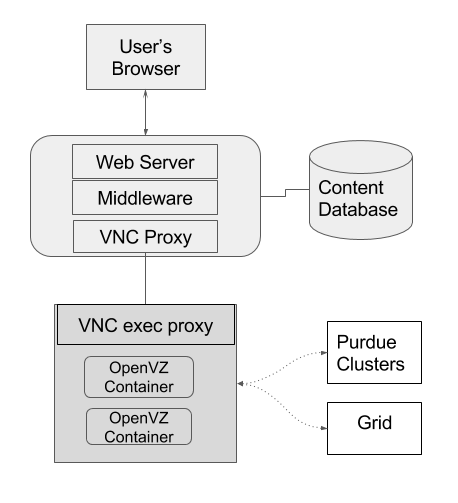
\includegraphics[width=1.5in]{arch_old}%
    \label{fig_arch_vnc}}
  \subfloat[Supports VNC and web applications]{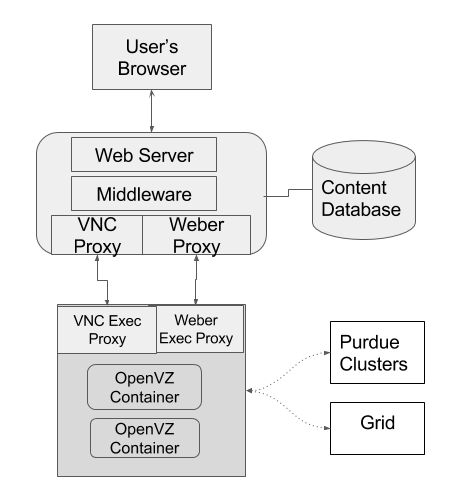
\includegraphics[width=1.5in]{arch_new}%
   \label{fig_arch_vnc_weber}}
  \caption{To support web applications, two new proxies needed to be added.
The Weber Front proxy, runs on the web server and terminates an SSL connection
between the user's web browser and the HUB. The Weber Exec proxy directs
connections to the tool container where the server side of web applications
 run.}
  \label{fig_arch}
\end{figure}



These challenges were first tackled for our initial implementation which made
Jupyter Notebooks available on the HUB. The implementation ran a notebook
server within the tool container and streamed HTML, CSS, and JavaScript from
the tool container, through the front and exec proxies, and out to the user's
web browser. Running the notebook server within the tool container give the web
application many of the same benefits of running a desktop style application in
the tool container. Namely, users could access their own HUB disk space, run
other applications that had been published on the HUB, and access powerful
compute clusters through Submit \cite{submit}. A similar setup was attempted
with the RStudio integrated development environment (IDE) and again with Wt, a
lesser known \CC based toolkit for building web applications. The robustness of
the new HUBzero architecture allowed each of these applications to be deployed
as web applications.

\section {Example web applications running on the HUB}

\subsection {Jupyter}

Jupyter is an open-source web application that allows you to create and share
documents that contain live code, equations, visualizations and explanatory
text. It includes an IDE that is expanding rapidly in capabilities. Common uses
include: data cleaning and transformation, numerical simulation, statistical
modeling, machine learning and much more.

Jupyter supports many different languages, but is primarily used for Python.
On HUBzero we currently also support R and Octave.

Jupyter content may be published as notebooks or as tools.  Notebooks are most
suitable for instructional content or workflows; where the user will be
interested in the implementation and may even modify its content while stepping
through the code cells.  Tools, on the other hand, have the code cells hidden.
Users may only interact with the exposed GUI elements. HUBzero extensions we
developed make it easier to use as an tool development framework.


\begin{figure}[!h]
	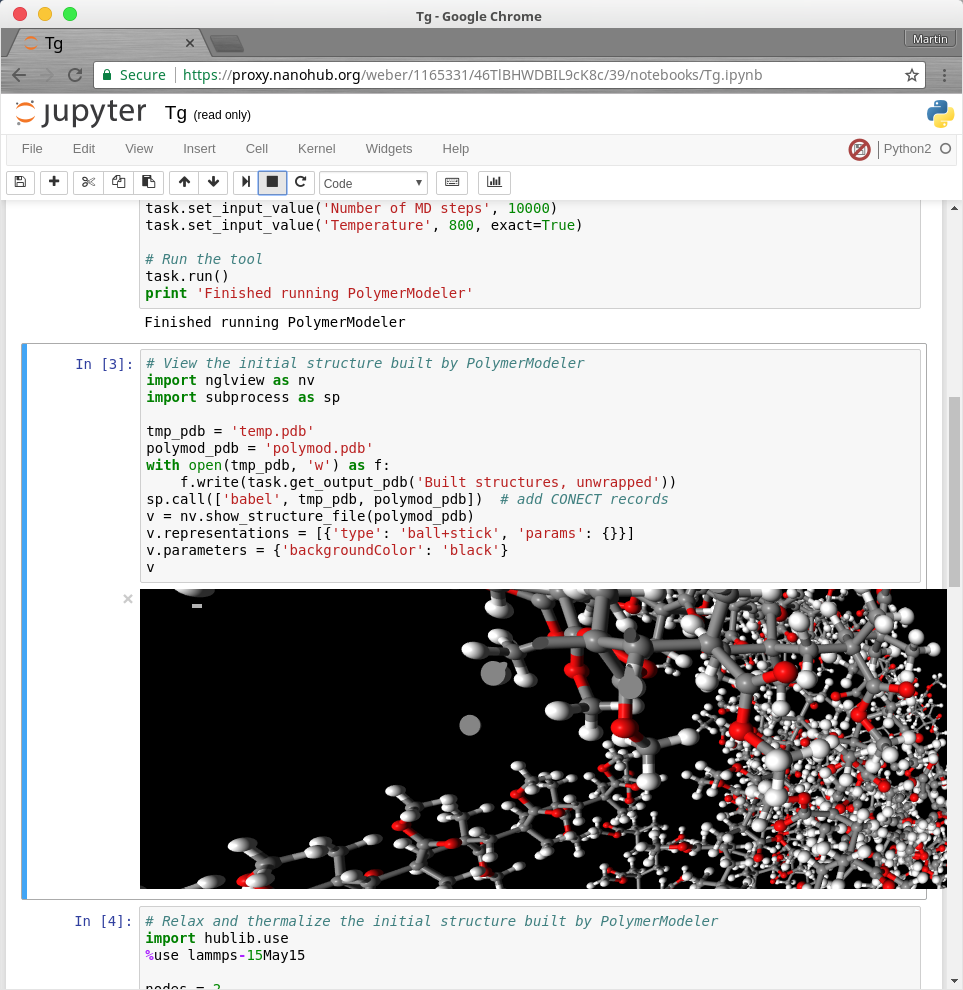
\includegraphics[width=3in]{tgnb}
	\caption{Glass Transition Notebook \cite{tg}}
	\label{fig_tg}
\end{figure}

An example of a notebook is shown in \Cref{fig_tg}.  This notebook calculate
the glass transition temperature of an atomistic, amorphous system by running
MD simulations in a notebook.  It does this by running a series of calculations
using Rappture tools and tools on clusters.

Note the lack of source code and editing tools in the Jupyter applications shown in
\Cref{fig_mdvacancy} and \Cref{fig_crack}.

\begin{figure}[!h]
	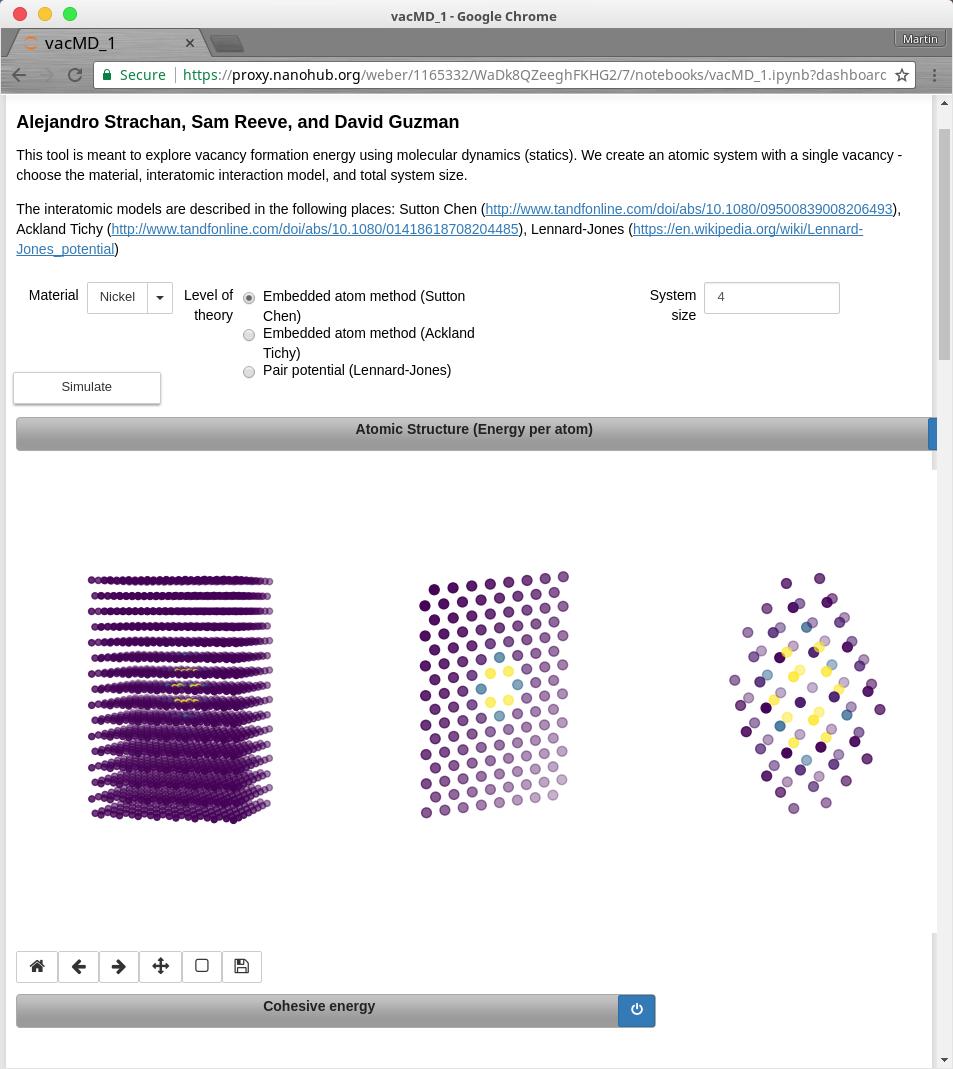
\includegraphics[width=3in]{mdvacancy}
	\caption{Vacancy Formation Energy with MD \cite{mdvacancy}}
	\label{fig_mdvacancy}
\end{figure}

\begin{figure}[!h]
	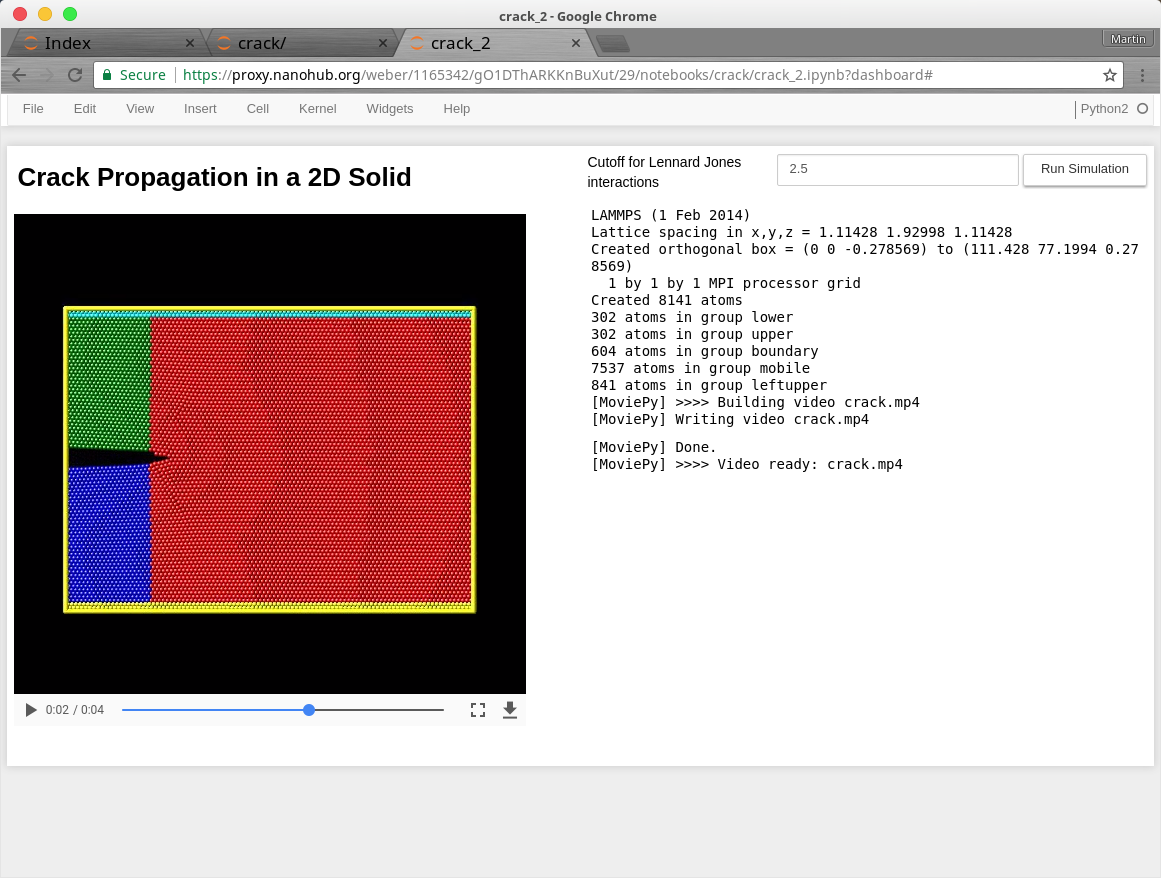
\includegraphics[width=3in]{crack}
	\caption{Creating a New Jupyter Tool}
	\label{fig_crack}
\end{figure}


\subsection {RStudio IDE, Shiny Applications, and RMarkdown Documents}

For many R users, RStudio is the graphical user interface of choice when
developing analysis and reports. The desktop version of the application
provides access to an R based integrated development environment (IDE) and is
available on all major platforms. RStudio Inc., the company behind the RStudio
IDE also makes available an Open Source web version of the application that can
be deployed on a server to provide access for multiple people at a time. While
the Open Source version of their IDE lacks the administrative, security, and
monitoring tools tools of their commercial version, it does provide many of the
features expected by users of the desktop version and can be a good replacement
for the desktop version if configured correctly.

Using the web version of the RStudio IDE on the HUB is a particularly good
match because the HUB's tool containers already provide the user space and
application space isolations that would be required of running a server like
this on a web server. Tool containers were developed with isolation and
resource management in mind.

On the HUB, when a user starts the RStudio application, the request is routed
from the user's web browser, through the HUB's webserver, front and exec
proxies, and into a tool container where an RStudio server waits to respond.

This same mechanism is used to support applications built using Shiny,
RStudio's library for building web applications from within R, and RMarkdown
documents. Like the RStudio IDE, Shiny applications and RMarkdown documents
require a web server to be running in the tool container to field requests from
the user's web browser. By themselves, static HTML documents with CSS and JavaScript
can also be served from within a tool container, but there is less of a need
for the isolation and security features provided by the tool container.

%%FIXME: add citations and examples of published rstudio apps.


\subsection {Other toolkits}

The changes made to the HUBzero Platform to support web applications are not
specific to supporting Jupyter Notebooks and RStudio's Shiny and RMarkdown
based applications and documents. The pattern of running a web server in the
tool container and connecting it to the user's web browser can be extended to
many of the web application frameworks available today. One library that
demonstrates this is Wt\cite{wt}. Wt is a \CC based library for building web
applications. Applications can be served using FastCGI in coordination with a
web server or the application can act as its own web server. The latter is
perfect for running in a tool container.

%%FIXME: add citations for Wt.



\section{Conclusion}
The landscape of web applications has changed dramatically over the last few
years. With the release of the HTML5 standard and the capabilities that are now
available, many developers are choosing to build interactive user interfaces
for their applications using HTML, CSS, and JavaScript. The HUBzero Platform
can now support these developers in the same way we have supported developers of
desktop applications. Furthermore, users of web development environments
like Jupyter Notebooks and RStudio have also grown and they are not only
interested in creating simulation tools and content, but also in sharing them.
With the changes we have made and outlined above, the HUB can now support these
new development environments.  As new technologies rise, the HUBzero team
continues to leverage its unique and flexible platform to serve as a resource
where people can develop, publish, and share their online simulations.



% references section

\begin{thebibliography}{1}

\bibitem{jupyter}
"Jupyter", \url{http://jupyter.org/}

\bibitem{rstudio}
"RStudio - Open Source and enterprise-ready professional software for R", \url{http://shiny.rstudio.com/}

\bibitem{openvz}
"OpenVZ Virtuozzo Containers", \url{https://openvz.org/}

\bibitem{rappture}
McLennan, M.; Kennell, R., \emph{HUBzero: A Platform for Dissemination
and Collaboration in Computational Science and Engineering}, Computing
in Science and Engineering, \textbf{12}(2):48-52 (2010).

\bibitem{submit}
M. McLennan, S. Clark, E. Deelman, M. Rynge, K. Vahi, F.
McKenna, D. Kearney, C. Song. \emph{HUBzero and Pegasus:
integrating scientific workflows into science gateways.} In
Concurrency and Computation: Practice and Experience,
2014; 27, pg 328-343, doi: 10.1002/cpe.3257

\bibitem{wt}
"Wt: \CC Web Toolkit", \url{https://www.webtoolkit.eu/wt}

\bibitem{tg}
Benjamin P Haley; Lorena Alzate-Vargas (2017), "Glass transition temperature notebook," https://nanohub.org/resources/tgnb. (DOI: 10.4231/D3N873142).

\bibitem{mdvacancy}
Sam Reeve (2017), "Vacancy Formation Energy with MD," https://nanohub.org/resources/mdvacancy. (DOI: 10.4231/D39S1KM5R).

\end{thebibliography}



\end{document}


